% \addtocontents{toc}{\protect\pagebreak}
\section{Mạng NeuMiss}

Để tính dự đoán Bayes trong phương trình \eqref{eq:mcar_bayes_predictor} và \eqref{eq:gaussian_bayes_predictor}, ta cần tính nghịch đảo của mỗi ma trận hiệp phương sai con $\cov_{obs(m)}$ với mỗi mẫu dữ liệu khuyết $m \in \{0,1\}^d$. Điều này tương đương với việc xây dựng một mô hình riêng biệt cho từng mẫu dữ liệu khuyết.

Với số lượng đơn vị ẩn (hidden units) tỷ lệ với $2^d$ mẫu dữ liệu khuyết, một mạng MLP với hàm kích hoạt (activation function) ReLU có thể học được các mô hình độc lập cho từng trường hợp. 
Tuy nhiên, khi số chiều $d$ lớn thì chi phí tính toán cũng trở nên lớn hơn. Các kiến trúc như MLP sẽ tạo ra số lượng tham số rất lớn vì chúng không chia sẻ thông tin giữa những mẫu dữ liệu khuyết tương tự nhau, nên chúng không tận dụng được mối quan hệ giữa các mẫu dữ liệu có đặc điểm khuyết giống nhau.

Một hướng tiếp cận khác là ước lượng vector $\mu$ và ma trận hiệp phương sai $\cov$ bằng thuật toán EM (Expectation Maximization), sau đó tính nghịch đảo của $\cov_{obs}$. Dẫu vậy, cách tiếp cận này cũng không hiệu quả do độ phức tạp tính toán tăng cao khi số chiều $d$ lớn.

Do đó, bài báo \cite{le2020neumiss} đề xuất một giải pháp trung hoà giữa 2 hướng trên: mô hình mối quan hệ giữa các hệ số cho các mẫu dữ liệu khuyết khác nhau thay vì ước lượng trực tiếp ma trận hiệp phương sai. Hiểu một cách trực quan, các dữ liệu quan sát được trong một mẫu sẽ được dùng để ước lượng tham số hồi quy cho các mẫu dữ liệu khác, thông qua việc chia sẻ tham số giữa các mẫu dữ liệu có đặc điểm chung. 

Trong mục này, ta sẽ xấp xỉ nghịch đảo của ma trận hiệp phương sai $\cov_{obs}$, tức xấp xỉ dự đoán Bayes bằng chuỗi Neumann, cũng như xét sự hội tụ của chuỗi và dự đoán Bayes. Với phép lặp xấp xỉ này, kết hợp với phương pháp Algorithm Unrolling \cite{gregor2010unroll}, ta sẽ có được một neural network mang tên NeuMiss (tiền tố Neu viết tắt cho Neumann và Neural network, Miss cho Missing). Mạng NeuMiss có thể tận dụng các tham số có thể học được trong mạng để xấp xỉ dự đoán Bayes, với các tham số được chia sẻ với nhau thông qua các mẫu dữ liệu khuyết, giúp giảm độ phức tạp tính toán và hiệu quả hơn.


\subsection{Xấp xỉ ma trận bằng chuỗi Neumann}
Thử thách lớn nhất của phương trình \eqref{eq:mcar_bayes_predictor} và \eqref{eq:gaussian_bayes_predictor} là việc tính nghịch đảo của ma trận $\cov_{obs(m)}$ với mọi $m \in \{0,1\}^d$. Khi $d$ lớn thì chi phí tính toán sẽ rất lớn.
Nên thay vì đi tính trực tiếp, bài báo đề xuất việc xấp xỉ nghịch đảo của $\cov_{obs(m)}$ một cách đệ quy bằng cách sử dụng chuỗi Neumann.

Đầu tiên, ta chọn 1 ma trận khởi tạo $S^{(0)}$ với $d \times d$ chiều. $S^{(0)}_{obs(m)}$ được định nghĩa là ma trận con của $S^{(0)}$, được tạo ra bằng cách chọn các cột và hàng sao cho dữ liệu không bị khuyết (các giá trị mà tại đó, $m = 0$)
và là xấp xỉ bậc-0 của $(\cov_{obs(m)})^{-1}$.
Sau đó, với mọi $m \in \{0,1\}^{d}$, ta định nghĩa xấp xỉ bậc-$\ell$ của $(\cov_{obs(m)})^{-1}$ qua phép lặp sau: Với mọi $\ell \geq 1$,
\begin{equation}\label{eq:iterative_fomula}
    S_{obs(m)}^{(\ell)} = (Id - \cov_{obs(m)}) S_{obs(m)}^{(\ell - 1)} + Id.
\end{equation}

Phép lặp $S_{obs(m)}^{(\ell)}$ hội tụ tuyến tính về $(\cov_{obs(m)})^{-1}$, và cũng là chuỗi Neumann chặt cụt tới~$\ell$ nếu $S^{(0)} = Id$.

\begin{proof}
    Ta xấp xỉ nghịch đảo ma trận $\cov_{obs(m)}$ bằng chuỗi Neumann:
    \[
        (\cov_{obs(m)})^{-1} = \sum_{k=0}^{\infty} (Id - \cov_{obs(m)})^k,
    \]
    tức 
    \[
        S^{}_{obs(m)} = \sum_{k=0}^{\infty} (Id - \cov_{obs(m)})^k.
    \]
    Chuỗi hội tụ khi $\|Id - \cov_{obs(m)}\|_2 < 1$. Vì bán kính phổ của $\cov$ nhỏ hơn $1$, nên bán kính phổ của mỗi ma trận con $\cov_{obs(m)}$ của $\cov$ cũng nhỏ hơn $1$, theo định lý Cauchy đan nhau (Cauchy Interlace Theorem) \cite{cauchyinterlacetheorem}, hoặc qua định nghĩa của các trị riêng dưới dạng tỷ số Rayleigh:
    \[
        \rho(\cov_{obs(m)}) 
        = \max_{\substack{u \in \R^{|obs(m)|}}} u^{\top} \cov_{obs(m)} u 
        = \max_{\substack{x \in \R^{d} \\ x_{mis}=0}} x^{\top} \cov x 
        \leq \max_{\substack{x \in \R^{d}}} x^{\top} \cov x 
        = \rho(\cov).
    \]
    
    Thay vì viết và tính toán dưới dạng chuỗi vô hạn, ta chỉ cần chuỗi xấp xỉ tới bậc-$\ell$:
    \[
        S^{(\ell)}_{obs(m)} = \sum_{k=0}^{\ell} (Id - \cov_{obs(m)})^k 
        = \sum_{k=0}^{\ell-1} (Id - \cov_{obs(m)})^k + (Id - \cov_{obs(m)})^{\ell}S^{(0)}_{obs(m)}.
    \]
    Với ma trận khởi tạo $S_{obs(m)}^{(0)}$, ta có thể định nghĩa một cách đệ quy thông qua phép lặp:
    \begin{equation*}
        S^{(\ell)}_{obs(m)} = (Id - \cov_{obs(m)} )S^{(\ell-1)}_{obs(m)} + Id \tag{\ref{eq:iterative_fomula}}.
    \end{equation*}

    Để rõ hơn, ta khai triển phương trình đệ quy trên:
    \begin{align*}
        S^{(\ell)}_{obs(m)} 
        &= (Id - \cov_{obs(m)})S^{(\ell-1)}_{obs(m)} + Id \\
        &= (Id - \cov_{obs(m)})((Id - \cov_{obs(m)})S^{(\ell-2)}_{obs(m)} + Id)  + Id \\
        &= (Id - \cov_{obs(m)})^2S^{(\ell-2)}_{obs(m)} + (Id - \cov_{obs(m)})  + Id \\
        &= (Id - \cov_{obs(m)})^3S^{(\ell-3)}_{obs(m)} + (Id - \cov_{obs(m)})^2 + (Id - \cov_{obs(m)})  + Id \\
        & \vdotswithin{=} \\[-10pt] % &\quad \vdots \\
        &= (Id - \cov_{obs(m)})^{\ell}S^{(0)}_{obs(m)} + \sum_{k=0}^{\ell-1}(Id - \cov_{obs(m)})^k.
    \end{align*}

    Ở \eqref{eq:iterative_fomula}, $(\cov_{obs(m)})^{-1}$ là điểm bất động của phương trình. Thật vậy:
    \begin{equation*}
        (\cov_{obs(m)})^{-1} = (Id - \cov_{obs(m)}) (\cov_{obs(m)})^{-1} + Id.
        % \label{eq:fixed_point_iteration}
    \end{equation*}
    Lấy phương trình này trừ đi \eqref{eq:iterative_fomula}, ta có:
    \[
        (\cov_{obs(m)})^{-1} - S^{\ell}_{obs(m)} = (Id - \cov_{obs(m)})((\cov_{obs(m)})^{-1} - S^{\ell-1}_{obs(m)}).
    \]

    Nhân $2$ vế phương trình trên cho $\cov_{obs(m)}$, ta được:
    \[
        Id - \cov_{obs(m)} S^{\ell}_{obs(m)} = (Id - \cov_{obs(m)})(Id -  \cov_{obs(m)} S^{\ell-1}_{obs(m)}).
    \]
    Lấy chuẩn $l_2$ (chuẩn phổ) cho cả $2$ vế và sử dụng bất đẳng thức Cauchy-Schwartz, ta được:
    \[
        \|Id - \cov_{obs(m)} S^{\ell}_{obs(m)} \|_2 \leq \|Id - \cov_{obs(m)}\|_2 \|Id -  \cov_{obs(m)} S^{\ell-1}_{obs(m)}\|_2.
    \]

    Cho $\nu_{obs(m)}$ là trị riêng nhỏ nhất của $\cov_{obs(m)}$, với giá trị dương do $\cov$ khả nghịch. Vì trị riêng của $\cov_{obs(m)}$ có chặn trên là $1$, ta có $\| Id - \cov_{obs(m)} \|_2 = (1 - \nu_{obs(m)})$. Bằng phép lặp đệ quy, ta nhận được:
    \begin{equation}\label{eq:iteration_converge_bound}
        \|Id - \cov_{obs(m)} S_{obs(m)}^{\ell}\|_2 
        \leq (1 - \nu_{obs(m)})^{\ell} \|Id - \cov_{obs(m)} S_{obs(m)}^{(0)}\|_2.
    \end{equation}
    

    Vậy $S_{obs(m)}^{(\ell)}$ hội tụ tuyến tính về $(\cov_{obs(m)})^{-1}$, và tốc độ hội tụ được xác định bởi trị riêng nhỏ nhất của $\cov_{obs(m)}$.  \qed
\end{proof}


Giờ ta đi định nghĩa xấp xỉ bậc-$\ell$ của dự đoán Bayes trong trường hợp cơ chế MAR (phương trình \eqref{eq:mcar_bayes_predictor}) dưới dạng:
\begin{equation}\label{eq:l_approximation_mcar_bayes_predictor}
    f_{\ell}^* (X_{obs}, M) = \langle\beta_{obs}^{*},X_{obs} \rangle+\langle\beta_{mis}^{*},\mu_{mis} + \cov_{mis,obs} S_{obs(m)}^{(\ell)}(X_{obs}-\mu_{obs})\rangle,
\end{equation}

Sai số giữa dự đoán Bayes và xấp xỉ bậc-$\ell$ của nó được cho bởi mệnh đề sau:
\begin{prop}\label{prop:error_approximation}
   Cho $\nu$ là trị riêng nhỏ nhất của $\cov$. Giả sử dữ liệu được sinh ra qua mô hình tuyến tính \eqref{eq:lr_matrix_notation} và tuân theo phân phối chuẩn đa biến. Giả sử giả thiết \ref{assume:mcar_assumption} hay \ref{assume:mar_assumption} thoả và bán kính phổ của $\cov$ nhỏ hơn $1$. Thì với mọi $\ell \geq 1$,
   \begin{equation}\label{eq:aprrox_error}
       \E \left[\left(f_{\ell}^* (X_{obs}, M) - f^* (X_{obs}, M)\right)^2\right] 
       \leq \dfrac{(1-\nu)^{2\ell} \|\beta^*\|_2^2}{\nu} \ \E\left[ \|Id - S_{obs(M)}^{(0)} \cov_{obs(M)}\|_2^2\right].
   \end{equation}
\end{prop}

% Mệnh đề này cung cấp chặn trên của sai số khi đi xấp xỉ $\cov_{obs(m)}^{-1}$.

\begin{proof}
    Với mệnh đề \ref{prop:mcar_bayes_predictor} và xấp xỉ bậc-$\ell$ cho dự đoán Bayes trong phương trình~\eqref{eq:l_approximation_mcar_bayes_predictor}, ta có:
    \[
        f_{\widetilde{X}, \ell}^* (\widetilde{X}) = 
        \langle\beta_{obs}^{*},X_{obs} \rangle + \langle\beta_{mis}^{*},\mu_{mis} + \cov_{mis,obs} S_{obs}^{(\ell)} (X_{obs}-\mu_{obs})\rangle.
    \]

    Do ta chỉ quan tâm tới phần xấp xỉ nên ta tạm thời bỏ qua $\beta^*_0$. Xét:
    \begin{align*}
        &\E [(f_{\widetilde{X}, \ell}^*(\widetilde{X}) - f_{\widetilde{X}}^* (\widetilde{X}))^2] \\
        &= \E \left[\langle\beta_{mis}^{*},\cov_{mis,obs} (S_{obs}^{(\ell)} - \cov_{obs}^{-1} ) (X_{obs}-\mu_{obs})\rangle^2\right]  \\
        &= \E \left[ (\beta_{mis}^{*})^{\top} \left(\cov_{mis,obs} (S_{obs}^{(\ell)} - \cov_{obs}^{-1} ) (X_{obs}-\mu_{obs})\right) 
        \left(\cov_{mis,obs} (S_{obs}^{(\ell)} - \cov_{obs}^{-1} ) (X_{obs}-\mu_{obs})\right)^{\top} \beta_{mis}^*\right]  \\
        &= \E \left[ (\beta_{mis}^{*})^{\top} \cov_{mis,obs} (S_{obs}^{(\ell)} - \cov_{obs}^{-1} ) (X_{obs}-\mu_{obs})
        (X_{obs}-\mu_{obs})^{\top} (S_{obs}^{(\ell)} - \cov_{obs}^{-1} )  \cov_{obs,mis} \beta_{mis}^*\right]  \\
        &= \E \left[ (\beta_{mis}^{*})^{\top} \cov_{mis,obs} (S_{obs}^{(\ell)} - \cov_{obs}^{-1} ) 
        \E[(X_{obs}-\mu_{obs}) (X_{obs}-\mu_{obs})^{\top} |M] (S_{obs}^{(\ell)} - \cov_{obs}^{-1} )  \cov_{obs,mis} \beta_{mis}^*\right]  \\
        &= \E \left[ (\beta_{mis}^{*})^{\top} \cov_{mis,obs} (S_{obs}^{(\ell)} - \cov_{obs}^{-1} ) 
        \cov_{obs} (S_{obs}^{(\ell)} - \cov_{obs}^{-1} )  \cov_{obs,mis} \beta_{mis}^*\right]  \\
        &= \E \left[ (\beta_{mis}^{*})^{\top} \cov_{mis,obs} (\cov_{obs} S_{obs}^{(\ell)} - Id_{obs} ) \cov_{obs}^{-1}
        \cov_{obs}^{\frac{1}{2}} \cov_{obs}^{\frac{1}{2}}
        \cov_{obs}^{-1}(\cov_{obs} S_{obs}^{(\ell)} - Id_{obs} )  \cov_{obs,mis} \beta_{mis}^*\right]  \\
        &= \E \left[ \big\| \cov_{obs}^{\frac{1}{2}}
        \cov_{obs}^{-1}(\cov_{obs} S_{obs}^{(\ell)} - Id_{obs} )  \cov_{obs,mis} \beta_{mis}^* \big\|_2^2 \right]  \\
        &= \E \left[ \big\| \cov_{obs}^{-\frac{1}{2}}
        ( Id_{obs} - \cov_{obs} S_{obs}^{(\ell)} )  \cov_{obs,mis} \beta_{mis}^* \big\|_2^2 \right].
    \end{align*}
    Với $
        \|\cov_{obs} x\|_2^2 = \sum_{i \in obs} (\cov_i^{\top} x)^2 \leq \sum_{i=1}^d (\cov_i^{\top} x)^2 = \|\cov x\|_2^2,
    $, tức $\|\cov_{obs} x\|_2 \leq \|\cov x\|_2$, 
    ta có:
    \[
        \|\cov_{obs, mis}\|_2 = \max_{\substack{\|x_{mis} \|_2 = 1}} \|\cov_{obs, mis} x_{mis}\|_2 
        \leq \max_{\substack{\|x\|_2 = 1 \\ x_{obs} = 0}} \|\cov_{obs} x\|_2
        \leq \max_{\substack{\|x\|_2 = 1 \\ x_{obs} = 0}} \|\cov x\|_2
        \leq \max_{\substack{\|x\|_2 = 1}} \|\cov x\|_2
        = \|\cov\|_2.
    \]
    Với trị riêng nhỏ nhất của $\cov$, ta có:
    \[
        \lambda_{\min}(\cov) = \min_{\substack{\|x\|_2=1}} x^{\top} \cov x 
        \leq \min_{\substack{\|x\|_2=1 \\ x_{mis}=0}} x^{\top} \cov x 
        = \min_{\|x_{obs}\|_2=1} x_{obs}^{\top} \cov_{obs} x_{obs} 
        = \lambda_{\min} (\cov_{obs}),
    \]
    mà $\|\cov^{-1}\|_2= \dfrac{1}{\lambda_{\min} (\cov) }$ 
    và $\|\cov_{obs}^{-1}\|_2 = \dfrac{1}{\lambda_{\min} (\cov_{obs})}$, 
    nên $\|\cov_{obs}^{-1}\|_2 \leq \|\cov^{-1}\|_2$.

    Do đó, ta được:
    \begin{align*}
        \E [(f_{\widetilde{X}, \ell}^*(\widetilde{X}) - f_{\widetilde{X}}^* (\widetilde{X}))^2] 
        &\leq \|\cov^{-1}\|_2 \|\cov\|_2^2 \|\beta^*\|_2^2
        \ \E\big[\| Id_{obs} - \cov_{obs} S_{obs}^{(\ell)}  \|_2^2 \big] \\
        &\leq \dfrac{1}{\nu}\|\beta^*\|_2^2 \ \E\big[(1 - \nu_{obs(m)})^{2\ell} \| Id_{obs} - \cov_{obs} S_{obs}^{(0)}  \|_2^2 \big] \quad \text{ (do \eqref{eq:iteration_converge_bound})}\\
        &= \dfrac{(1 - \nu_{obs(m)})^{2\ell}\|\beta^*\|_2^2 }{\nu} \ \E\big[ \| Id_{obs} - \cov_{obs} S_{obs}^{(0)}  \|_2^2 \big].
    \end{align*}
    
    Vậy ta có điều phải chứng minh.   \qed
\end{proof}

Mệnh đề \ref{prop:error_approximation} cho biết: 
Sai số của xấp xỉ bậc-$\ell$ phân rã (decay), hay tiến về $0$ rất nhanh theo hàm mũ khi $\ell$ tăng. Quan trọng hơn, nếu ma trận con $S^{(0)}_{obs(m)}$ của $S^{(0)}$ là một xấp xỉ tốt của $\cov_{obs}^{-1}$, 
nghĩa là nếu ta chọn $S^{(0)}$ để tối thiểu hoá kỳ vọng ở vế bên phải của bất đẳng thức \eqref{eq:aprrox_error}, thì mô hình của chúng ta sẽ cung cấp một xấp xỉ tốt cho dự đoán Bayes ngay cả khi bậc $\ell = 0$.
 Điều này đúng với ma trận hiệp phương sai dạng đường chéo, vì việc chọn $S^{(0)} = \cov^{-1}$ không có sai số xấp xỉ, do $(\cov^{-1})_{obs} = (\cov_{obs})^{-1}$.


\subsection{Kiến trúc của mạng NeuMiss}
Bài báo \cite{le2020neumiss} đề xuất một kiến trúc neural network có tên là NeuMiss để xấp xỉ dự đoán Bayes, với nghịch đảo $\cov_{obs}^{-1}$ được tính toán bằng một phiên bản được ``unroll'' của phép lặp Neumann. Hình \ref{fig:neumiss} cho ta kiến trúc của neural network sử dụng xấp xỉ bậc-$3$, tương ứng với độ sâu $4$. Với $x$ là dữ liệu đầu vào, giá trị bị khuyết được thay bằng $0$, và $\mu$ là tham số có thể huấn luyện (trainable) tương ứng với $\mu$ ở trong phương trình xấp xỉ bậc-$\ell$ của dự đoán Bayes \eqref{eq:l_approximation_mcar_bayes_predictor}:
\[
    f_{\ell}^* (X_{obs}, M) = \langle\beta_{obs}^{*},X_{obs} \rangle+\langle\beta_{mis}^{*},\mu_{mis} + \cov_{mis,obs} S_{obs(m)}^{(\ell)}(X_{obs}-\mu_{obs})\rangle,
\]

Để giống với dự đoán Bayes (phương trình 
\eqref{eq:l_approximation_mcar_bayes_predictor}), 
ma trận trọng số (weight matrix) $W$ là một phép biến đổi đơn giản của \textcolor{blue}{ma trận hiệp phương sai} như trong hình \ref{fig:neumiss}.


\begin{figure}[h]
    \centering
    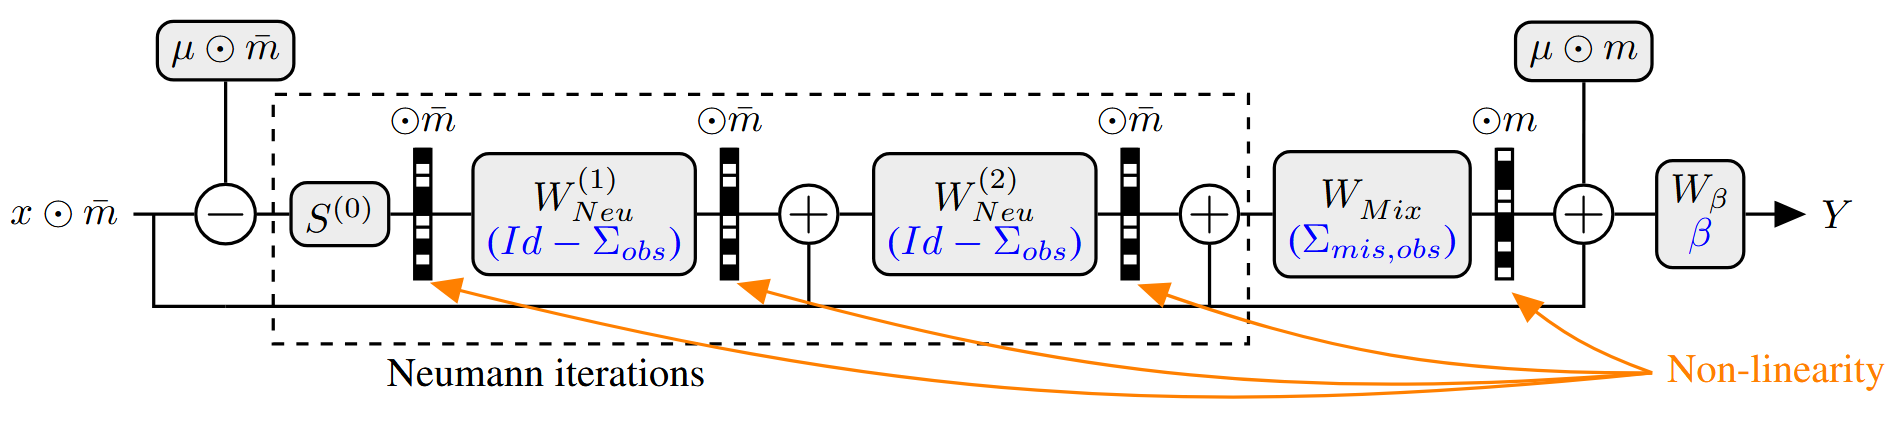
\includegraphics[width=\textwidth]{img/neumiss_network.png}
    \caption{
        \textbf{Kiến trúc mạng NeuMisss với độ sâu $4$} --- $\bar{m} = 1 - m$. Mỗi ma trận trọng số $W^{(k)}$ tương ứng với một phép biến đổi của \textcolor{blue}{ma trận hiệp phương sai}.
    }
    \label{fig:neumiss}
\end{figure}


Mỗi phép lặp Neumann đi qua một ma trận trọng số, qua tất cả $W^{(k)}_{Neu}$. Hay đúng hơn là ta học mỗi lớp một cách độc lập, theo như bài báo về Algorithm Unrolling \cite{gregor2010unroll} đã đề cập, khi mà các trọng số của các lớp có thể cải thiện hiệu quả xấp xỉ của mô hình.

Các trị số cho các giá trị quan sát được thay đổi với mỗi mẫu dữ liệu, nên 
có thể dẫn tới khó khăn trong việc cài đặt. 
Ví dụ như dữ liệu bị khuyết với mẫu $m$, ma trận trọng số $S^{(0)}, W_{Neu}^{(1)}, W_{Neu}^{(2)}$ của hình \ref{fig:neumiss} nên được masked sao cho các hàng và cột tương ứng với các trị số $mis(m)$ có giá trị bằng $0$, và các hàng của $W_{Mix}$ tương ứng với $obs(m)$ cũng như các cột của $W_{Mix}$ tương ứng với $mis(m)$ có giá trị bằng $0$.

Triển khai neural network với ma trận trọng số được masked theo các cách khác nhau với mỗi mẫu dữ liệu có thể phức tạp, nên bài báo đề xuất cách làm sau: Cho $W$ là ma trận trọng số, $v$ là một vector, và $\bar{m} = 1 - m$. Lúc này, $(W\odot \bar{m} \bar{m}^{\top}) v = (W(v \odot \bar{m}))\odot \bar{m}$, nghĩa là sử dụng ma trận trọng số được masked tương đương với việc masking vector đầu vào và đầu ra. Mạng NeuMiss có thể được xem là một neural network truyền thống với các hàm kích hoạt phi tuyến là \textbf{tích của các mask với nhau}. Cách tiếp cận này khiến việc cài đặt trở nên đơn giản hơn và cải thiện tốc độ tính toán của neural network, cũng như dễ dàng diễn giải hơn khi các mask điều khiển các thông tin của dữ liệu bị khuyết khi mạng được huấn luyện.

Theo như lý thuyết, chuỗi Neumann cần phải được lặp nhiều lần mới cho ra kết quả xấp xỉ nghịch đảo tốt, nên mạng NeuMiss cần phải sâu vì mỗi lớp tượng trưng cho 1 phép lặp. Do đó, mạng cần phải có residual connection, giúp model học được tốt hơn khi số lượng lớp nhiều.
Mặc dù sau khi thực nghiệm, việc có hay không có residual connection không ảnh hưởng quá nhiều đến hiệu suất của mạng NeuMiss (xem \ref{section:residual_connection}).


\textbf{Xấp xỉ trong trường hợp Gaussian self-masking}

Mặc dù kiến trúc mạng NeuMiss được xây dựng dựa trên dự đoán Bayes trong trường hợp MCAR và MAR, nhưng nó cũng có thể được sử dụng cho cơ chế self-masking~\eqref{eq:gaussian_bayes_predictor}. Giả sử $D_{mis} \cov_{mis|obs}^{-1} \approx Id$, thì dự đoán Bayes cho self-masking trở thành:
\begin{align*}
    f^*(X_{obs}, M) 
    &\approx \beta_{0}^{*} + \langle\beta_{obs}^{*}, X_{obs}\rangle 
    + \langle\beta_{mis}^{*},(2Id)^{-1} (\tilde{\mu}_{mis} + Id(\mu_{mis} + \cov_{mis,obs}\left(\cov_{obs}\right)^{-1} (X_{obs}-\mu_{obs}))) \rangle \\
    &\approx \beta_{0}^{*} + \langle\beta_{obs}^{*}, X_{obs}\rangle 
    + \langle\beta_{mis}^{*}, \frac{1}{2}(\tilde{\mu}_{mis} + \mu_{mis} + \cov_{mis,obs}\left(\cov_{obs}\right)^{-1} (X_{obs}-\mu_{obs})) \rangle \\
    &\approx \beta_0^* + \langle \beta_{obs}^*, X_{obs}\rangle + \langle \beta_{mis}^*, \frac{1}{2} (\widetilde{\mu}_{mis} + \mu_{mis}) + \frac{1}{2}  \cov_{mis,obs} (\cov_{obs})^{-1} (X_{obs} - \mu_{obs}) \rangle.
\end{align*}

Phương trình này giống như phương trình dự đoán Bayes cho cơ chế M(C)AR \eqref{eq:mcar_bayes_predictor}, nhưng với $\mu_{mis}$ được thay bởi $\frac{1}{2} (\widetilde{\mu}_{mis} + \mu_{mis})$ và $\cov_{mis,obs}$ trở thành $\frac{1}{2}\cov_{mis,obs}$. Dưới phép xấp xỉ này, dự đoán Bayes cho cơ chế self-masking có thể được mô hình bởi kiến trúc được đề xuất. Điểm khác biệt duy nhất là giá trị được quan tâm là tham số $\mu$ và $W_{mix}$ của mạng.

Một phép xấp xỉ khác cũng phù hợp cho dự đoán Bayes: $D_{mis} \cov_{mis|obs}^{-1} \approx \hat{D}_{mis}$ khi $\hat{D}$ là một ma trận ma trận đường chéo. Trong trường hợp này, kiến trúc được đề xuất có thể mô hình dự đoán Bayes cho self-masking:
\begin{multline*}
    f^*(X_{obs}, M) 
    \approx \beta_0^* + \langle \beta_{obs}^*, X_{obs}\rangle + \langle \beta_{mis}^*, 
    (Id + \hat{D}_{mis})^{-1} (\widetilde{\mu}_{mis} + \hat{D}_{mis} \mu_{mis}) \\
    + (Id + \hat{D}_{mis})^{-1} \hat{D}_{mis} \cov_{mis,obs} (\cov_{obs})^{-1} (X_{obs} - \mu_{obs}) \rangle.
\end{multline*}

Ở đây, tham số $\mu$ của mạng nhắm tới $(Id + \hat{D}_{mis})^{-1} (\widetilde{\mu}_{mis} + \hat{D}_{mis} \mu_{mis})$ và $W_{mix}$ nhắm tới $(Id + \hat{D}_{mis})^{-1} \hat{D}_{mis} \cov_{mis,obs}$ thay vì chỉ là $\cov_{mis,obs}$ trong trường hợp M(C)AR. Do đó, kiến trúc được đề xuất có thể xấp xỉ tốt dự đoán Bayes trong trường hợp self-masking bằng cách điều chỉnh giá trị tham số $\mu$ và $W_{mix}$ học được nếu $D_{mis} \cov_{mis|obs}^{-1}$ gần giống với ma trận đường chéo.



%-------------------------------------------------
% \section{Liên kết với MLP và hàm kích hoạt ReLU}
% % Multilayer Perceptron với hàm kích hoạt là 
% % hàm ReLU có dạng:
% % \begin{equation}
% %     \relu(x) = \max(x, 0).
% % \end{equation}

% % nhân các mask lại với nhau

% % Connections to Other Architectures:  A shallow (depth-1) NeuMiss network exhibits a close relationship to a Multilayer Perceptron (MLP) with ReLU activation that operates on the concatenated vector of imputed data and the mask.  This connection suggests that the commonly used MLP with an imputed mask can be interpreted as a simplified instance of a NeuMiss network.

% Một quy tắc thường dùng khi xử lý dữ liệu khuyết đó là xem dữ liệu đầu vào là ghép (concatenate) của dữ liệu với mask dữ liệu khuyết. Do  
% % the pattern of missing data itself may carry useful information for predictive models.
% các mẫu dữ liệu khuyết có thể cung cấp các thông tin hữu ích cho mô hình dự đoán.
% Mệnh đề tiếp theo liên kết quy tắc này với mạng NeuMiss.

% \begin{prop}(Mạng NeuMiss-1 layer tương đương với MLP)\label{prop:neumiss-mlp}
%     \newline
%     Cho $[X \odot (1-M), M] \in [0,1]^d \times \{0,1\}^d$ là dữ liệu đầu vào $X$ được điền khuyết bởi giá trị $0$ ghép với mask $M$.

%     \begin{itemize}
%         \item Cho $\mathcal{H}_{\relu} = (W \in \R^{d \times 2d}, \relu)$ là một hidden layer (layer ẩn) liên kết $[X \odot (1-M), M]$ với $d$ hidden units, và áp dụng hàm kích hoạt phi tuyến $\relu$.
%         \item Cho $\mathcal{H}_{\odot M} = (W \in \R^{d \times d}, \mu, \odot M)$ là một hidden layer liên kết $(X - \mu) \odot (1 - M)$ với $d$ hidden units, và áp dụng hàm kích hoạt phi tuyến $\odot M$.
%     \end{itemize}
%     Ký hiệu $h^{\relu}_{k}$ và $h^{\odot M}_{k}$ tượng trưng cho kết quả đầu ra của hidden unit thứ $k^{th}$ của mỗi layer. Thì tồn tại một tuỳ chỉnh của ma trận trọng số của hidden layer $\mathcal{H}_{\relu}$ sao cho $\mathcal{H}_{\odot M}$ và $\mathcal{H}_{\relu}$ có cùng hidden units kích hoạt cho bất kì $(X_{obs}, M)$, và hidden units được kích hoạt có dạng $h_{k}^{\relu}(X_{obs}, M) = h_{k}^{\odot M} (X_{obs}, M) + c_k$, với $c_k \in \R$.
% \end{prop}

% Mệnh đề 
% % \ref{prop:neumiss-mlp} 
% trên
% chỉ ra rằng, một hidden layer $\mathcal{H}_{\relu}$ có thể được viết lại như là một layer $\mathcal{H}_{\odot M}$ cộng với $1$ hằng số. Khi $1$ layer khác được thêm vào sau $\mathcal{H}_{\odot M}$ hay $\mathcal{H}_{\relu}$, hằng số này có thể được coi như là bias của layer mới này. Do đó, các trọng số của $\mathcal{H}_{\relu}$ có thể được học để giống với $\mathcal{H}_{\odot M}$. Trong trường hợp này, nó có nghĩa là một MLP với hàm kích hoạt \relu, với một hidden layer cho $d$  hidden units, hoạt động trên vector ghép với mask, thì giống với lại mạng NeuMiss với độ sâu là $1$ (Hình \ref{fig:neumiss}), do đó cung cấp một nền tảng lý thuyết cho việc sử dụng các mạng MLP sau mạng NeuMiss.

% \begin{proof}
%     Phần chứng minh có ở trong phần phụ lục A.7 của bài báo.
% \end{proof}
